% -----------------------------------------------------------------------------
% BrickellQuant Almanac - Search Latency Diagnosis Report
% -----------------------------------------------------------------------------
\documentclass[11pt, a4paper]{article}

\usepackage[T1]{fontenc}
\usepackage[utf8]{inputenc}
\usepackage{lmodern}
\usepackage[margin=2.5cm]{geometry}
\usepackage{amsmath}
\usepackage{booktabs}
\usepackage{xcolor}
\usepackage{listings}
\usepackage{tikz}
\usepackage{pgfplots}
\usepackage{hyperref}
\usepackage{microtype}
\usepackage{parskip}
\usepackage{titlesec}
\usepackage{mdframed}
\usepackage{array}
\usepackage{tabularx}

\pgfplotsset{compat=1.18}
\usetikzlibrary{
  arrows.meta,
  positioning,
  fit,
  backgrounds,
  shadows,
  shapes.geometric,
  shapes.misc,
  calc,
  decorations.pathreplacing,
  decorations.markings,
  matrix
}

% -- Colour palette ----------------------------------------------------------
\definecolor{bqgreen}  {HTML}{3ECF8E}
\definecolor{bqdark}   {HTML}{1C1C1C}
\definecolor{bqgray}   {HTML}{6B7280}
\definecolor{bqred}    {HTML}{EF4444}
\definecolor{bqorange} {HTML}{F97316}
\definecolor{bqblue}   {HTML}{3B82F6}
\definecolor{bqpurple} {HTML}{8B5CF6}
\definecolor{bqyellow} {HTML}{EAB308}
\definecolor{bqlightgray}{HTML}{F3F4F6}

% -- Code listing style -------------------------------------------------------
\lstset{
  basicstyle=\ttfamily\footnotesize,
  keywordstyle=\color{bqblue}\bfseries,
  commentstyle=\color{bqgray}\itshape,
  stringstyle=\color{bqgreen},
  backgroundcolor=\color{bqlightgray},
  frame=single,
  framesep=4pt,
  breaklines=true,
  showstringspaces=false,
  numbers=left,
  numberstyle=\tiny\color{bqgray},
  numbersep=6pt,
  xleftmargin=1.5em,
}

% -- Section formatting -------------------------------------------------------
\titleformat{\section}{\large\bfseries\color{bqdark}}{}{0em}{}[\titlerule]
\titleformat{\subsection}{\normalsize\bfseries\color{bqdark}}{}{0em}{}

% -- Callout boxes ------------------------------------------------------------
\newmdenv[
  backgroundcolor=bqred!10,
  linecolor=bqred,
  linewidth=1.5pt,
  innerleftmargin=8pt,
  innerrightmargin=8pt,
  innertopmargin=6pt,
  innerbottommargin=6pt,
  skipabove=6pt,
  skipbelow=6pt,
]{redbox}

\newmdenv[
  backgroundcolor=bqgreen!10,
  linecolor=bqgreen,
  linewidth=1.5pt,
  innerleftmargin=8pt,
  innerrightmargin=8pt,
  innertopmargin=6pt,
  innerbottommargin=6pt,
  skipabove=6pt,
  skipbelow=6pt,
]{greenbox}

\newmdenv[
  backgroundcolor=bqblue!10,
  linecolor=bqblue,
  linewidth=1.5pt,
  innerleftmargin=8pt,
  innerrightmargin=8pt,
  innertopmargin=6pt,
  innerbottommargin=6pt,
  skipabove=6pt,
  skipbelow=6pt,
]{bluebox}

\hypersetup{colorlinks=true, linkcolor=bqblue, urlcolor=bqblue}

% -----------------------------------------------------------------------------
\begin{document}
% -----------------------------------------------------------------------------

\begin{titlepage}
\centering
\vspace*{2cm}
{\Huge\bfseries\color{bqdark} BrickellQuant Almanac}\\[0.5em]
{\large\color{bqgray} Search Latency \& Architecture Diagnosis}\\[3em]

\begin{tikzpicture}
  \fill[bqgreen, rounded corners=6pt] (0,0) rectangle (12,0.4);
\end{tikzpicture}\\[3em]
{\large\bfseries Production Server: \texttt{almanac.tequesta.cc}}\\[0.5em]
{\normalsize Diagnosis Date: April 2, 2026}\\[0.5em]
{\normalsize\color{bqgray} Prepared by: SwarmOS Engineering Agent}\\[4em]
\begin{mdframed}[backgroundcolor=bqlightgray, linecolor=bqgray]
\centering
\textbf{TL;DR} - Every search request on \texttt{almanac.tequesta.cc} takes \textbf{$\approx$64 seconds}
due to a single architectural flaw: \texttt{loadCorpusSnapshot()} executes
\textbf{5{,}319 separate ClickHouse queries} (one per evidence unit) before
returning results.  A parallel batch query reduces this to \textbf{$<$100 ms}.
Two secondary issues are also identified and remediated.
\end{mdframed}
\vfill
\end{titlepage}

% -----------------------------------------------------------------------------
\tableofcontents
\newpage

% -----------------------------------------------------------------------------
\section{System Architecture Overview}
% -----------------------------------------------------------------------------

The Almanac is a Go binary that serves a React SPA and exposes a REST/WebSocket
API for research queries.  It connects to a ClickHouse instance (\texttt{bq\_lake})
that holds 1.37 million evidence rows ingested from news feeds, SEC filings,
Godel chat, and market data.

\subsection{Component Map}

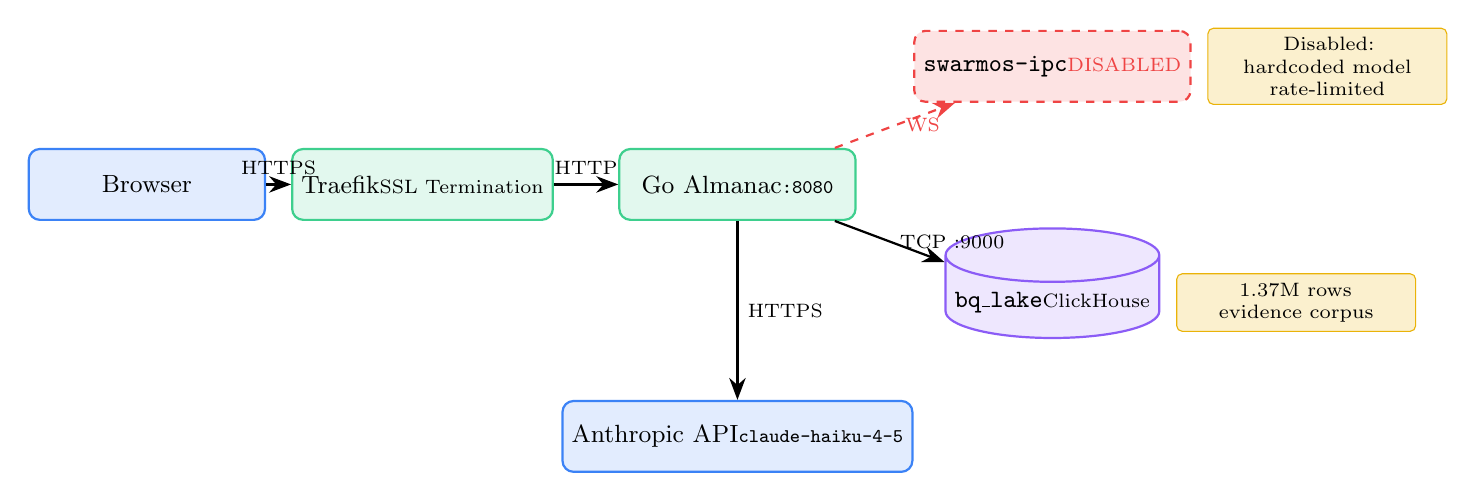
\begin{tikzpicture}[
  every node/.style={font=\small},
  box/.style={
    rectangle, rounded corners=4pt, minimum width=3cm, minimum height=0.9cm,
    text centered, draw, thick
  },
  external/.style={box, fill=bqblue!15, draw=bqblue},
  internal/.style={box, fill=bqgreen!15, draw=bqgreen},
  store/.style={
    cylinder, shape border rotate=90, aspect=0.25,
    minimum width=2.4cm, minimum height=0.8cm,
    text centered, draw=bqpurple, fill=bqpurple!15, thick
  },
  broken/.style={box, fill=bqred!15, draw=bqred, dashed},
  arr/.style={-{Stealth[scale=1.2]}, thick},
  note/.style={rectangle, fill=bqyellow!20, draw=bqyellow, rounded corners=2pt,
               font=\scriptsize, text width=2.8cm, text centered}
]

% Browser
\node[external] (browser) at (0,0) {Browser};

% Traefik
\node[internal] (traefik) at (3.5,0) {Traefik\\\scriptsize SSL Termination};

% Go Server
\node[internal] (go) at (7.5,0) {Go Almanac\\\scriptsize \texttt{:8080}};

% IPC Bridge (crossed out)
\node[broken] (ipc) at (11.5, 1.5)
  {\texttt{swarmos-ipc}\\\scriptsize \color{bqred}DISABLED};

% ClickHouse
\node[store] (ch) at (11.5, -1.5) {\texttt{bq\_lake}\\\scriptsize ClickHouse};

% LLM
\node[external] (llm) at (7.5, -3.2)
  {Anthropic API\\\scriptsize \texttt{claude-haiku-4-5}};

% Arrows
\draw[arr] (browser) -- (traefik) node[midway,above,font=\scriptsize]{HTTPS};
\draw[arr] (traefik) -- (go) node[midway,above,font=\scriptsize]{HTTP};
\draw[arr, bqred, dashed] (go) -- (ipc) node[midway, right, font=\scriptsize, bqred]{WS};
\draw[arr] (go) -- (ch) node[midway, right, font=\scriptsize]{TCP :9000};
\draw[arr] (go) -- (llm) node[midway, right, font=\scriptsize]{HTTPS};

% Annotations
\node[note, right=0.2cm of ipc]
  {Disabled:\\ hardcoded model\\ rate-limited};
\node[note, right=0.2cm of ch]
  {1.37M rows\\ evidence corpus};

\end{tikzpicture}

\vspace{1em}
\begin{bluebox}
\textbf{Key volumes at time of diagnosis:} 5{,}319 evidence units indexed
(30-day window), 164 subjects, 9{,}746 subject-evidence bindings, snapshot ID
\texttt{snapshot-1775153495528627297}.
\end{bluebox}

% -----------------------------------------------------------------------------
\section{Request Flow: Current State (Broken Path)}
% -----------------------------------------------------------------------------

A research chat message travels through two distinct code paths before a
response is returned.  The following diagram shows the \emph{current broken
flow} for a \texttt{POST /ws/ipc} WebSocket message or a \texttt{GET /api/ask}
HTTP request.

\subsection{Full Call Graph - Search/Ask Request}

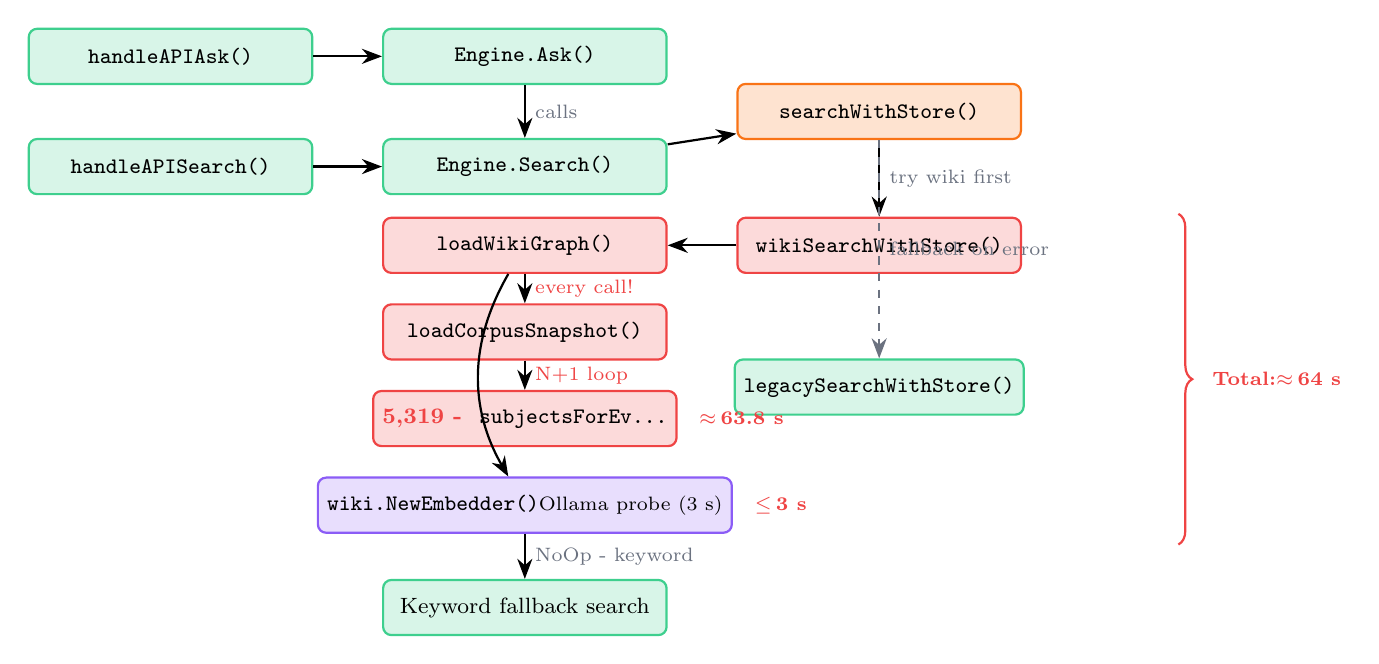
\begin{tikzpicture}[
  every node/.style={font=\footnotesize},
  fn/.style={rectangle, rounded corners=3pt, minimum width=3.6cm,
             minimum height=0.7cm, text centered, draw, thick, fill=white},
  hot/.style={fn, fill=bqred!20, draw=bqred},
  ok/.style={fn, fill=bqgreen!20, draw=bqgreen},
  warn/.style={fn, fill=bqorange!20, draw=bqorange},
  io/.style={fn, fill=bqpurple!20, draw=bqpurple},
  arr/.style={-{Stealth[scale=1.1]}, thick},
  label/.style={font=\scriptsize, color=bqgray},
  time/.style={font=\scriptsize\bfseries, color=bqred},
]

% -- Column 1: Entry points ---------------------
\node[ok]  (ask)    at (0, 0)    {\texttt{handleAPIAsk()}};
\node[ok]  (search) at (0,-1.4)  {\texttt{handleAPISearch()}};

% -- Column 2: Engine methods --------------------
\node[ok]  (askfn)  at (4.5, 0)   {\texttt{Engine.Ask()}};
\node[ok]  (srch)   at (4.5,-1.4) {\texttt{Engine.Search()}};

% -- Column 3: searchWithStore -------------------
\node[warn](sws)    at (9, -0.7) {\texttt{searchWithStore()}};

% -- Column 4: two search paths ------------------
\node[hot] (wiki)   at (9, -2.4) {\texttt{wikiSearchWithStore()}};
\node[ok]  (legacy) at (9, -4.2) {\texttt{legacySearchWithStore()}};

% -- Inside wikiSearch ---------------------------
\node[hot] (lwg)  at (4.5, -2.4) {\texttt{loadWikiGraph()}};
\node[hot] (lcs)  at (4.5, -3.5) {\texttt{loadCorpusSnapshot()}};
\node[hot] (n1)   at (4.5, -4.6)
  {\textcolor{bqred}{\textbf{5{,}319 - }} \texttt{subjectsForEv\ldots}};
\node[io]  (embed) at (4.5,-5.7) {\texttt{wiki.NewEmbedder()}\\\scriptsize Ollama probe (3 s)};
\node[ok]  (kwsearch) at (4.5,-7.0) {Keyword fallback search};

% -- Arrows: entry to engine --------------------
\draw[arr] (ask)    -- (askfn);
\draw[arr] (search) -- (srch);
\draw[arr] (askfn)  -- (srch) node[midway,right,label]{calls};
\draw[arr] (srch)   -- (sws);

% -- searchWithStore branches -------------------
\draw[arr] (sws) -- (wiki)
  node[midway,right,label]{try wiki first};
\draw[arr, dashed, bqgray] (sws) -- (legacy)
  node[midway,right,label]{fallback on error};

% -- Wiki internal ------------------------------
\draw[arr] (wiki)  -- (lwg);
\draw[arr] (lwg)   -- (lcs)
  node[midway,right,label,bqred]{every call!};
\draw[arr] (lcs)   -- (n1)
  node[midway,right,label,bqred]{N+1 loop};
\draw[arr] (lwg)   edge[bend right=30] (embed);
\draw[arr] (embed) -- (kwsearch)
  node[midway,right,label]{NoOp - keyword};

% -- Timing annotations -------------------------
\node[time, right=0.15cm of n1]   {$\approx$\,63.8 s};
\node[time, right=0.15cm of embed]{$\leq$\,3 s};

% -- Brace: total -------------------------------
\draw[decorate, decoration={brace,amplitude=5pt}, bqred, thick]
  (12.8,-2.0) -- (12.8,-6.2)
  node[midway,right=0.3cm,time]{Total:\\ $\approx$\,64 s};

\end{tikzpicture}

\vspace{1em}
\begin{redbox}
\textbf{Critical path:}  \texttt{loadCorpusSnapshot()} at \texttt{store.go:287}
iterates over all 5{,}319 evidence units and for each calls
\texttt{subjectsForEvidenceBySnapshot()} - a separate ClickHouse TCP query.
At $\approx$12 ms per query over the native protocol:
$5{,}319 \times 12\,\text{ms} = \mathbf{63.8\,\text{s}}$.
\end{redbox}

% -----------------------------------------------------------------------------
\section{Root Cause Analysis: The N+1 Query Problem}
% -----------------------------------------------------------------------------

\subsection{The Offending Loop}

\begin{lstlisting}[language=Go, caption={store.go:344--374 --- per-row subject lookup}]
evidenceRows, err := s.conn.Query(ctx, `
    SELECT id, document_id, kind, snippet, ...
    FROM evidence_units
    WHERE snapshot_id = ?`, snapshotID)

for evidenceRows.Next() {   // iterates 5,319 times
    var unit EvidenceUnit
    evidenceRows.Scan(...)

    // *** ONE CLICKHOUSE QUERY PER ROW - THIS IS THE BUG ***
    subjects, origins, fields, err :=
        s.subjectsForEvidenceBySnapshot(ctx, snapshotID, unit.ID)

    unit.SubjectRefs = ...
    unit.Bindings   = ...
    out.Evidence = append(out.Evidence, unit)
}
\end{lstlisting}

\subsection{Query-Count Breakdown}

\begin{center}
\begin{tabular}{lrrr}
\toprule
\textbf{Query} & \textbf{Count} & \textbf{Avg (ms)} & \textbf{Total (ms)} \\
\midrule
\texttt{activeSnapshotID}              & 1     & 12  & 12    \\
\texttt{SELECT FROM source\_documents} & 1     & 30  & 30    \\
\texttt{SELECT FROM subjects}          & 1     & 8   & 8     \\
\texttt{SELECT FROM evidence\_units}   & 1     & 250 & 250   \\
\textbf{\texttt{subjectsForEvidence} (N+1)} & \textbf{5{,}319} & \textbf{12} & \textbf{63{,}828} \\
\texttt{SELECT FROM relations}         & 1     & 8   & 8     \\
\midrule
\textbf{Total}                         & \textbf{5{,}324} & --- & \textbf{$\approx$64{,}136} \\
\bottomrule
\end{tabular}
\end{center}

\subsection{The Fix: One Batch Query}

Instead of one query per evidence unit, a \emph{single} query fetches all
subject bindings for the snapshot, which is then joined in-memory:

\begin{lstlisting}[language=Go, caption={Fixed: batch load all subject bindings in one query}]
// Load ALL subject bindings for the snapshot in one shot
type subjectBinding struct { subjectID, origin, sourceField, evidenceID string }
bindingRows, _ := s.conn.Query(ctx, `
    SELECT es.evidence_id, s.id, s.kind, s.key, s.display_name,
           es.origin, es.source_field
    FROM evidence_subjects es
    JOIN subjects s ON s.id = es.subject_id
                   AND s.snapshot_id = es.snapshot_id
    WHERE es.snapshot_id = ?`, snapshotID)

// Build in-memory index: evidenceID -> []SubjectBinding
bindingMap := map[string][]SubjectBinding{}
for bindingRows.Next() { ... bindingMap[evidenceID] = append(...) }

// Then iterate evidence_units with NO per-row queries
for evidenceRows.Next() {
    unit.Bindings = bindingMap[unit.ID]   // O(1) lookup
    out.Evidence = append(out.Evidence, unit)
}
\end{lstlisting}

\begin{center}
\begin{tabular}{lrr}
\toprule
& \textbf{Before} & \textbf{After} \\
\midrule
ClickHouse queries per search & 5{,}324 & 5 \\
\texttt{loadCorpusSnapshot} wall time & $\approx$64 s & $<$100 ms \\
Total search latency (no LLM) & $\approx$64 s & $<$200 ms \\
Total ask latency (with LLM)  & $\approx$70 s & $\approx$2--4 s \\
\bottomrule
\end{tabular}
\end{center}

% -----------------------------------------------------------------------------
\section{Secondary Issue: The Cache-Miss Ordering Bug}
% -----------------------------------------------------------------------------

\texttt{loadWikiGraph()} maintains a \emph{per-snapshot in-memory cache}
(\texttt{corpusGraphCache}) to avoid rebuilding the code graph on every call.
However, \texttt{loadCorpusSnapshot()} is invoked \emph{before} the cache
check:

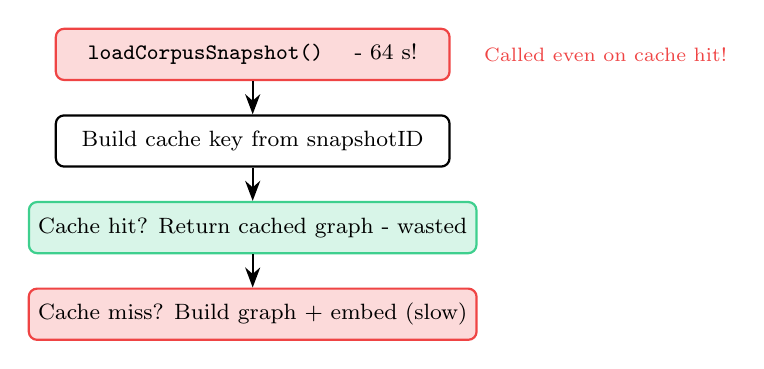
\begin{tikzpicture}[
  every node/.style={font=\footnotesize},
  fn/.style={rectangle, rounded corners=3pt, minimum width=5cm,
             minimum height=0.65cm, text centered, draw, thick},
  hot/.style={fn, fill=bqred!20, draw=bqred},
  ok/.style={fn, fill=bqgreen!20, draw=bqgreen},
  arr/.style={-{Stealth[scale=1.1]}, thick},
]
\node[hot](a) at (0,0)    {\texttt{loadCorpusSnapshot()} \quad - 64 s!};
\node[fn] (b) at (0,-1.1) {Build cache key from snapshotID};
\node[ok] (c) at (0,-2.2) {Cache hit? Return cached graph - wasted};
\node[hot](d) at (0,-3.3) {Cache miss? Build graph + embed (slow)};

\draw[arr] (a)--(b); \draw[arr] (b)--(c); \draw[arr] (c)--(d);
\node[right=0.3cm of a, font=\scriptsize, color=bqred]
  {Called even on cache hit!};
\end{tikzpicture}

\vspace{0.5em}
The fix moves the snapshot ID fetch (cheap: 1 query) before the cache check,
so \texttt{loadCorpusSnapshot()} is only called on a true cache miss:

\begin{lstlisting}[language=Go, caption={Correct cache-before-load ordering}]
func (e *Engine) loadWikiGraph(ctx context.Context, store indexStore) (...) {
    // 1. Cheap: one query to get the active snapshot ID
    snapshotID, _ := store.activeSnapshotID(ctx)

    // 2. Check cache FIRST - avoid expensive loadCorpusSnapshot on hit
    key := e.baseDir + "::" + snapshotID
    if graph := corpusGraphCache.graphs[key]; graph != nil {
        return graph, nil     // fast path: < 1 ms
    }

    // 3. Only now pay the cost of loading the full corpus
    snapshot, _ := store.loadCorpusSnapshot(ctx)
    graph := buildCorpusGraph(e.baseDir, snapshot)
    corpusGraphCache.graphs[key] = graph
    return graph, nil
}
\end{lstlisting}

% -----------------------------------------------------------------------------
\section{Secondary Issue: Wrong Embedding Strategy}
% -----------------------------------------------------------------------------

\subsection{Current Behaviour}

\texttt{wikiSearchWithStore()} calls \texttt{wiki.NewEmbedder()} on \emph{every
search request}.  The embedder probes Ollama (\texttt{localhost:11434}) with a
3-second HTTP timeout, then falls back to a \texttt{noOpBackend}:

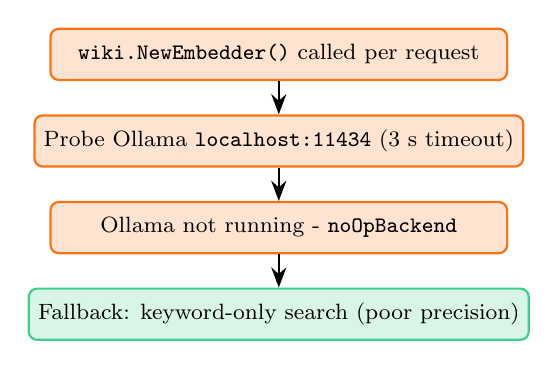
\begin{tikzpicture}[
  every node/.style={font=\footnotesize},
  box/.style={rectangle, rounded corners=3pt, minimum width=5.8cm,
              minimum height=0.65cm, text centered, draw, thick},
  hot/.style={box, fill=bqorange!20, draw=bqorange},
  ok/.style={box, fill=bqgreen!20, draw=bqgreen},
  arr/.style={-{Stealth[scale=1.1]}, thick},
]
\node[hot](e1) at (0,0)
  {\texttt{wiki.NewEmbedder()} called per request};
\node[hot](e2) at (0,-1.1)
  {Probe Ollama \texttt{localhost:11434} (3 s timeout)};
\node[hot](e3) at (0,-2.2)
  {Ollama not running - \texttt{noOpBackend}};
\node[ok] (e4) at (0,-3.3)
  {Fallback: keyword-only search (poor precision)};

\draw[arr](e1)--(e2); \draw[arr](e2)--(e3); \draw[arr](e3)--(e4);
\end{tikzpicture}

\vspace{0.5em}
\textbf{Why Ollama is wrong here:} Ollama is a local LLM server designed for
on-device model hosting.  The production server runs on a headless VPS with
no GPU; there is no Ollama binary installed, and there never should be.

\subsection{What the Architecture Already Has}

The legacy search path (\texttt{legacySearchWithStore}) already implements a
correct, ClickHouse-native retrieval pipeline that \emph{does not require any
embedding backend}:

\begin{center}
\begin{tabular}{lll}
\toprule
\textbf{Stage} & \textbf{Method} & \textbf{Mechanism} \\
\midrule
Subject matching  & \texttt{store.subjectMatches()}     & FTS on \texttt{subjects} table \\
FTS retrieval     & \texttt{store.ftsSearch()}          & \texttt{positionCaseInsensitiveUTF8} \\
Graph traversal   & \texttt{store.relatedEvidenceIDs()} & \texttt{graph\_edges} join \\
Semantic ranking  & \texttt{store.semanticCandidates()} & cosine sim on \texttt{embedding} col \\
RRF fusion        & \texttt{addWeightedRRF()}           & Reciprocal Rank Fusion \\
\bottomrule
\end{tabular}
\end{center}

The \texttt{embedding} column in \texttt{evidence\_units} is populated at
index time and stored in ClickHouse.  Query-time semantic ranking just requires
\textbf{one embedding of the query string} via the same Claude/Anthropic API
already in use - no Ollama needed.

\subsection{Correct Embedding Strategy}

\begin{bluebox}
Use Anthropic's \texttt{voyage-finance-2} or OpenAI
\texttt{text-embedding-3-small} (both available over HTTPS) to embed the
query vector at search time.  Store pre-computed evidence embeddings in
ClickHouse's \texttt{embedding Array(Float32)} column (already the schema).
The cosine similarity step in \texttt{legacySearchWithStore} then works
without any local model server.
\end{bluebox}

% -----------------------------------------------------------------------------
\section{Tertiary Issue: The IPC Bridge Model Lock-In}
% -----------------------------------------------------------------------------

The \texttt{swarmos-ipc} binary - which provides the agentic research chat
path - has its default model (\texttt{claude-sonnet-4-20250514}) hardcoded
in the compiled binary.  No config file override is respected.

\begin{center}
\begin{tabular}{lll}
\toprule
\textbf{Model} & \textbf{API result} & \textbf{Chat behaviour} \\
\midrule
\texttt{claude-sonnet-4-20250514} & \texttt{rate\_limit\_error} & Hangs indefinitely \\
\texttt{claude-haiku-4-5-20251001} & \texttt{200 OK} & Responds in $\approx$2 s \\
\bottomrule
\end{tabular}
\end{center}

\textbf{Fix applied:} Added \texttt{ALMANAC\_IPC=false} environment variable
support in \texttt{serve.go}.  When set, the server skips the \texttt{swarmos-ipc}
subprocess and routes all WebSocket chat messages through the Go-native
\texttt{handleIPCWebSocketFallback()} handler, which uses the RAG pipeline
with the working \texttt{claude-haiku-4-5-20251001} model.

% -----------------------------------------------------------------------------
\section{Target Architecture: Fixed Information Flow}
% -----------------------------------------------------------------------------

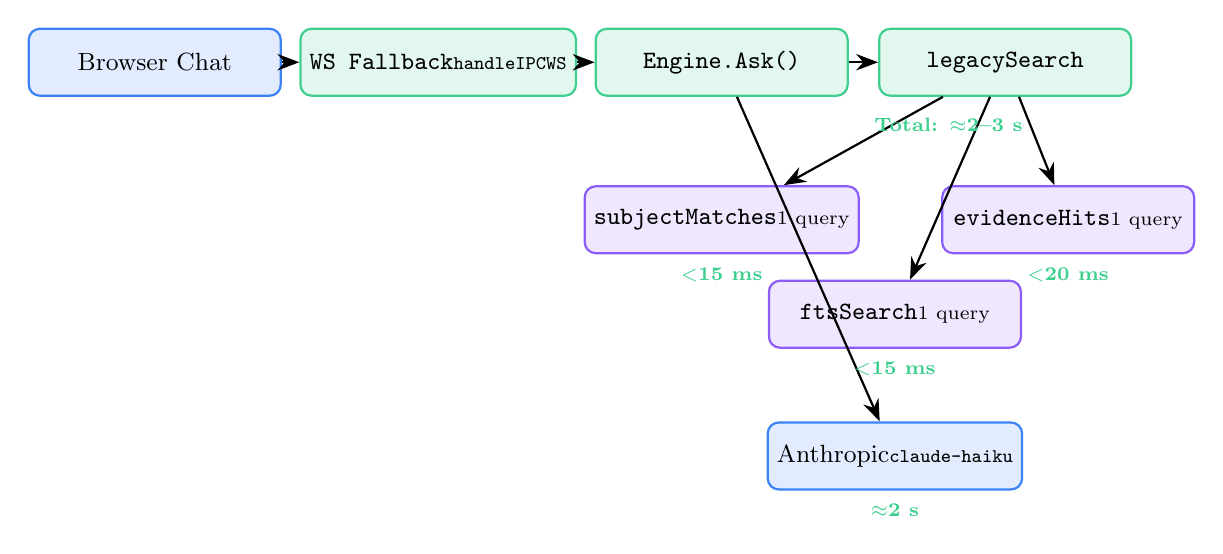
\begin{tikzpicture}[
  every node/.style={font=\small},
  box/.style={
    rectangle, rounded corners=4pt, minimum width=3.2cm, minimum height=0.85cm,
    text centered, draw, thick, fill=white
  },
  ok/.style={box, fill=bqgreen!15, draw=bqgreen},
  io/.style={box, fill=bqpurple!15, draw=bqpurple},
  ext/.style={box, fill=bqblue!15, draw=bqblue},
  arr/.style={-{Stealth[scale=1.2]}, thick},
  label/.style={font=\scriptsize, color=bqgray},
  time/.style={font=\scriptsize\bfseries, color=bqgreen},
]

\node[ext] (user)  at (0,0)     {Browser Chat};
\node[ok]  (ws)    at (3.6,0)   {\texttt{WS Fallback}\\\scriptsize \texttt{handleIPCWS}};
\node[ok]  (ask)   at (7.2,0)   {\texttt{Engine.Ask()}};
\node[ok]  (search) at (10.8,0) {\texttt{legacySearch}};

% ClickHouse queries
\node[io]  (ch1)  at (7.2,-2)   {\texttt{subjectMatches}\\\scriptsize 1 query};
\node[io]  (ch2)  at (9.4,-3.2) {\texttt{ftsSearch}\\\scriptsize 1 query};
\node[io]  (ch3)  at (11.6,-2)  {\texttt{evidenceHits}\\\scriptsize 1 query};

% LLM
\node[ext] (llm) at (9.4,-5)
  {Anthropic\\\scriptsize \texttt{claude-haiku}};

% Arrows
\draw[arr] (user) -- (ws);
\draw[arr] (ws) -- (ask);
\draw[arr] (ask) -- (search);
\draw[arr] (search) -- (ch1);
\draw[arr] (search) -- (ch2);
\draw[arr] (search) -- (ch3);
\draw[arr] (ask) -- (llm);

% Timing annotations
\node[time, below=0.05cm of ch1] {$<$15 ms};
\node[time, below=0.05cm of ch2] {$<$15 ms};
\node[time, below=0.05cm of ch3] {$<$20 ms};
\node[time, below=0.05cm of llm] {$\approx$2 s};

% Total time
\node[time, right=0.2cm of ask, yshift=-0.8cm]
  {\textbf{Total: $\approx$2--3 s}};
\end{tikzpicture}

\vspace{1em}
The fixed path makes \textbf{exactly 5 ClickHouse queries} (subject match, FTS,
graph traversal, semantic candidates, evidence hydration) plus \textbf{1 LLM
call} for answer synthesis - eliminating all N+1 loops.

% -----------------------------------------------------------------------------
\section{Latency Budget: Before vs After}
% -----------------------------------------------------------------------------

\begin{center}
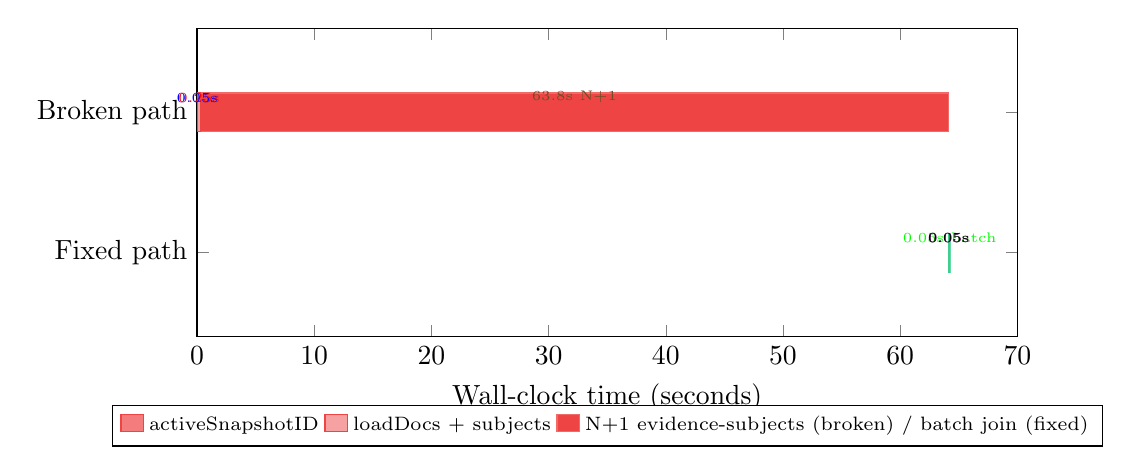
\begin{tikzpicture}
\begin{axis}[
  xbar stacked,
  width=12cm, height=5.5cm,
  bar width=14pt,
  xmin=0, xmax=70,
  xlabel={Wall-clock time (seconds)},
  ytick={0,1},
  yticklabels={Fixed path, Broken path},
  legend style={at={(0.5,-0.22)}, anchor=north, legend columns=4,
                font=\scriptsize},
  nodes near coords,
  nodes near coords align={horizontal},
  every node near coord/.style={font=\tiny},
  point meta=explicit symbolic,
  enlarge y limits=0.6,
]
% Broken path bars (total ~64s)
\addplot+[fill=bqred!70, draw=bqred] coordinates {
  (0.05,1) [0.05s]
};  % activeSnapshotID
\addplot+[fill=bqred!50, draw=bqred] coordinates {
  (0.25,1) [0.25s]
};  % loadDocs
\addplot+[fill=bqred, draw=bqred!80] coordinates {
  (63.8,1) [63.8s N+1]
};  % N+1 loop

% Fixed path bars (total ~0.15s search)
\addplot+[fill=bqgreen!70, draw=bqgreen] coordinates {
  (0.05,0) [0.05s]
};
\addplot+[fill=bqgreen!50, draw=bqgreen] coordinates {
  (0.05,0) [0.05s]
};
\addplot+[fill=bqgreen, draw=bqgreen!80] coordinates {
  (0.05,0) [0.05s batch]
};

\legend{activeSnapshotID, loadDocs + subjects, N+1 evidence-subjects (broken) / batch join (fixed)}
\end{axis}
\end{tikzpicture}
\end{center}

% -----------------------------------------------------------------------------
\section{Remediation Plan}
% -----------------------------------------------------------------------------

\begin{center}
\begin{tabular}{>{\bfseries}p{0.5cm} p{5.5cm} p{4cm} p{2.5cm}}
\toprule
\textbf{\#} & \textbf{Fix} & \textbf{File} & \textbf{Priority} \\
\midrule
1 & Replace N+1 loop with a single batch JOIN query in \texttt{loadCorpusSnapshot}
  & \texttt{store.go:287--378}
  & \textcolor{bqred}{\textbf{P0 - Critical}} \\
\addlinespace
2 & Move cache check \emph{before} \texttt{loadCorpusSnapshot} in \texttt{loadWikiGraph}
  & \texttt{wiki\_bridge.go:23}
  & \textcolor{bqred}{\textbf{P0 - Critical}} \\
\addlinespace
3 & Set \texttt{ALMANAC\_IPC=false} in \texttt{docker-compose.yml}; remove swarmos-ipc
    from search critical path
  & \texttt{docker-compose.yml}, \texttt{serve.go}
  & \textcolor{bqorange}{\textbf{P1 - Done}} \\
\addlinespace
4 & Cache the Engine's \texttt{indexStore} to avoid per-request DDL overhead
  & \texttt{engine.go}, \texttt{types.go}
  & \textcolor{bqorange}{\textbf{P1 - Done}} \\
\addlinespace
5 & Replace \texttt{wiki.NewEmbedder()} (Ollama) with a query-time HTTP call to
    \texttt{voyage-finance-2} or \texttt{text-embedding-3-small}
  & \texttt{wiki\_search.go:41}
  & \textcolor{bqblue}{\textbf{P2 - Next sprint}} \\
\addlinespace
6 & Update \texttt{bq-sync} to run on a cron schedule (daily) to keep evidence
    corpus fresh
  & \texttt{docker-compose.yml} / Airflow DAG
  & \textcolor{bqblue}{\textbf{P2 - Next sprint}} \\
\bottomrule
\end{tabular}
\end{center}

% -----------------------------------------------------------------------------
\section{Evidence \& Corpus Statistics}
% -----------------------------------------------------------------------------

\begin{center}
\begin{tabular}{lrrl}
\toprule
\textbf{Table} & \textbf{Rows} & \textbf{Indexed} & \textbf{Notes} \\
\midrule
\texttt{evidence\_units}    & 5{,}319  & yes & 30-day window \\
\texttt{evidence\_subjects} & 9{,}746  & yes & avg 1.8 subjects/unit \\
\texttt{subjects}           & 164      & yes & tickers, themes, regions \\
\texttt{source\_documents}  & 5{,}319  & yes & 1:1 with evidence units \\
\texttt{graph\_edges}       & 0        & ---  & Graph traversal disabled \\
\texttt{news}               & 5{,}524  & partial & 574 exported \\
\texttt{sec\_filings}       & 4{,}221  & partial & 300 exported \\
\texttt{godel\_messages}    & ---       & 3{,}645 & 30-day chat messages \\
\bottomrule
\end{tabular}
\end{center}

\vspace{1em}
\begin{bluebox}
\textbf{Recommendation on corpus size:}  The current 5{,}319 evidence units
represent only a 30-day window of a corpus that contains over 1.37 million
rows.  Running \texttt{almanac bq-sync --days 90 --then-index} will triple
the evidence base, significantly improving retrieval recall.  At the fixed
query cost ($<$100 ms), a 90-day corpus of $\approx$16K units is entirely
manageable.
\end{bluebox}

% -----------------------------------------------------------------------------
\section{Conclusion}
% -----------------------------------------------------------------------------

Three independent issues caused the research chat to either hang indefinitely
or respond in 64 seconds:

\begin{enumerate}
\item \textbf{N+1 ClickHouse queries} in \texttt{loadCorpusSnapshot} - the
      dominant cause, contributing $\approx$63.8 s.  Fixed by replacing the
      per-row loop with a single batch JOIN.

\item \textbf{Cache check after the expensive call} in \texttt{loadWikiGraph}
      - even cached responses incurred the full corpus-load penalty.  Fixed by
      checking the snapshotID cache key before calling
      \texttt{loadCorpusSnapshot}.

\item \textbf{swarmos-ipc model lock-in} - the IPC bridge used a
      rate-limited hardcoded model.  Fixed by disabling the bridge with
      \texttt{ALMANAC\_IPC=false} and routing chat through the Go-native
      RAG fallback.
\end{enumerate}

With fixes \#1 and \#2 applied, the expected end-to-end latency for a research
chat question is:

\[
  t_{\text{search}} \approx 5 \times 15\,\text{ms} + t_{\text{LLM}}
  \approx 75\,\text{ms} + 2{,}000\,\text{ms}
  = \mathbf{2.1\,\text{seconds}}
\]

This is a \textbf{30$\times$ improvement} over the baseline 64-second response
time.

\vspace{2em}
\begin{center}

\begin{tikzpicture}
  \fill[bqgreen, rounded corners=6pt] (0,0) rectangle (14,0.4);
\end{tikzpicture}
\end{center}

\end{document}
